%%%%%%%%%%%%%%%%%%%%%%%%%%%%%%%%%%%%%%%%%%%%%%%%%%%%%%%%%%%%%%%%%%%%%%%%%%%%%
%	e-Yantra, IIT-Bombay

%	Document Author: Abhishek rathore, Gopineedi Harsha Vardhan
%	Date: 8-June,2016 

%%%%%%%%%%%%%%%%%%%%%%%%%%%%%%%%%%%%%%%%%%%%%%%%%%%%%%%%%%%%%%%%%%%%%%%%%%%%%

\documentclass[11pt,a4paper]{article}

\usepackage{graphicx}
\usepackage{caption}
\usepackage{subcaption}
\usepackage{url}
\usepackage{hyperref}
\graphicspath{{../Images/}}
\title{Interfacing the Camera and Gimbal system with the R-Pi}
\author{e-Yantra Team}
\date{\today}

\begin{document}
	\maketitle
	\newpage
	\tableofcontents
	\newpage
	\section{Interfacing the Camera and Gimbal system with the R-Pi}
	\textbf{Objective} of this tutorial is to interface the desired camera(PiCam/USB Camera)and the Gimbal system(Servos) with the Raspberry-Pi and install the essential packages on the R-Pi board 
	\section{Prerequisites}
	\begin{itemize}
		\item A RaspbianOS installed Raspberry-Pi 
		\item Python and Open CV installed on the R-Pi
	\end{itemize}
	\section{Hardware Requirement}
	\begin{itemize}
		\item Raspberry-Pi B+ Development Board
		\item Raspberry-Pi Camera Module(Pi Camera)
		\item Ethernet Cable/Wifi Mdoule
		\item Tower-Pro Micro Servos 9gm(2 No.)
		\item 3-D printed Camera fixing mount
		\item Connecting wires
		\item External power supply(if needed)
	\end{itemize}
	\section{Software Requirement}
	\begin{itemize}
		\item OpenCV 2.4.1
		\item Python 2.7
		\item MobaXterm 9.0
	\end{itemize}
	\section{Setup}
		
		\subsection{Setting up Raspberry-Pi}
		\par We will be using the Raspberry-Pi remotely from our Laptop/PC using SSH connection by MobaXterm using a LAN Cable or by a Wi-fi module that is setup on the Pi.Make sure that the Pi is connected to the Internet as we need to install necessary packages for further setup.
		\par In our case,we connected to the Pi through LAN by assigning it a static IP from the "cmdline.txt" file on the SD card.We are accessing the Internet through the Wi-fi module.
		\par It is also possible to overclock the R-Pi externally through the "config.txt" file from the SD card or internally through the "/boot/config" file.The need for overclocking is to meet the excessive processing needs of our Gimbal system.(Although it is not recommended as it may cause heating problems).
		\par In our case,we overclocked the R-Pi from 700 Mhz(default) to 900 Mhz.
		
		\subsection{Setting up Camera(Pi-Cam)}
		After fixing the Pi-cam in its connector located between the Ethernet port and HDMI port,boot up your Raspberry-Pi and open the terminal and run the following command and enable the camera(if not enabled) and reboot ur R-Pi.
		\begin{center}
			
\includegraphics[scale=0.6]{cmd.png}
		\end{center}
		\begin{center}
		   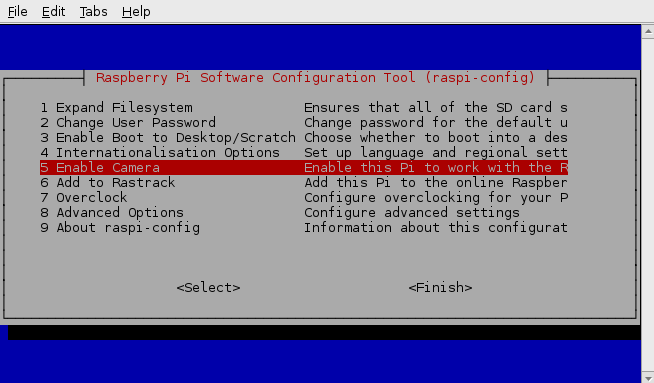
\includegraphics[scale=0.6]{enablecam.png}
		\end{center}
		\par We can check the working status of the camera by using "raspistill -o image.jpg" which takes a picture with the camera and stores it in image.jpg. 
	
		\subsection{Setting up the Pan-Tilt System}
		For making the Pan-Tilt system we will be using Two Tower Pro Servo Motors each weighing 9g (we used micro servos as they would draw a little amount of current which can be produced by the R-Pi itself)
		  \begin{center}
		   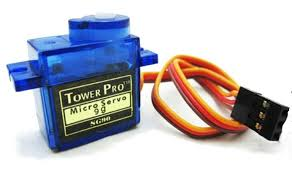
\includegraphics[scale=0.5]{servo.jpg}
		\end{center}
		\par We connected the first servo to the Pin 16(GPIO 23) and second servo to Pin 18(GPIO 24) on the board.We use this pins as signal channels when we use the servos from R-Pi.All the available GPIO ports that can be used are shown below.
		 \begin{center}
		   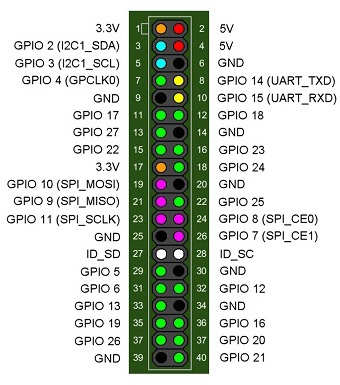
\includegraphics[scale=0.6]{gpio.jpg}
		\end{center}
		\par We calibrated each of the motor's PWM values(explained in the later section) and assembled to the frame mount which is shown below.
		  \begin{center}
		   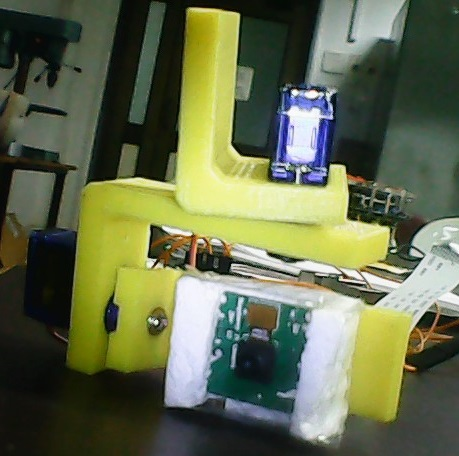
\includegraphics[scale=0.6]{frame.jpg}
		\end{center}
		
			
	\section{Necessary Packages}
    These are the packages that need to be installed in python for using the Pan-Tilt system.
	 \begin{itemize}
	 \item OpenCV
	 \item picamera
	 \item picamera-array
	 \item RPIO
	 \end{itemize}
		
	\section{Calibrating the Servos}
	 After installing the RPIO package we can calibrate the servos accordingly.Open the                       Terminal and run Python and import RPIO package and run the following.
	   \begin{center}
		   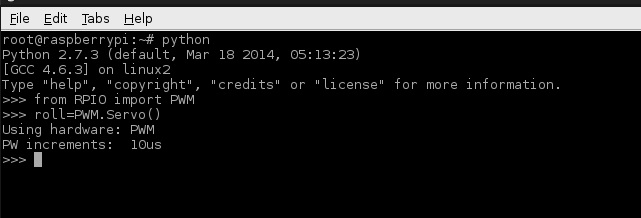
\includegraphics[scale=0.6]{cmd2.jpg}
		\end{center}
		
We check the angle of the servo of at different values of PWM given to it.In our case we got 0 degree between 500 and 600 and 180 degree between 2300 and 2400.After some calibrations we got 90 degree at 1520.
	 \begin{center}
		   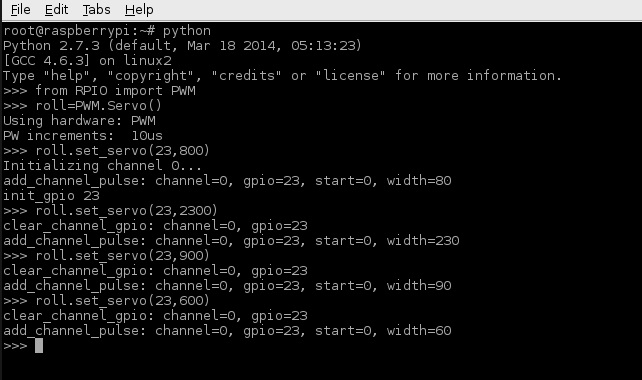
\includegraphics[scale=0.6]{cmd3.jpg}
		\end{center}
	 \par After the calibration,we assembled the Servos at 90 degree to the frame and making it a Pan-Tilt System.Here we used an external Powerbank(2 Amp) as a power supply to the R-pi.(Current requirement of the servos is more)
	  \begin{center}
		   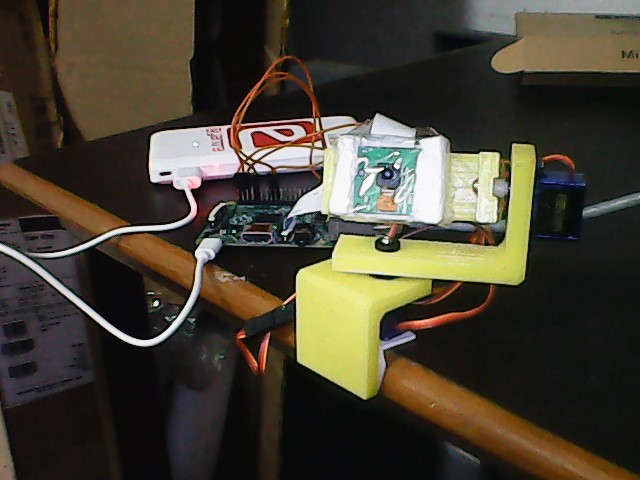
\includegraphics[scale=0.6]{image.jpg}
		\end{center}
	 
	 \section{References}
	\begin{itemize}
		\item \url{https://www.raspberrypi.org/help/camera-module-setup/}
		\item \url{https://thepihut.com/blogs/raspberry-pi-tutorials/16021420-how-to-install_use-the-raspberry-pi-camera}
		\item \url{http://cmucam.org/projects/cmucam5/wiki/Assembling_pantilt-Mechanism}
		\item \url{https://www.youtube.com/watch?v=2LltXMHVuDs}
	\item \url{https://www.raspberrypi.org/documentation/usage/gpio/}	
	\item \url{https://www.raspberrypi.org/blog/using-the-gpio/}	
	\end{itemize}
\end{document}